\setcounter{page}{3}
\chapter{Теоретическая часть}

\section{Задание}

Цель работы: построение гистограммы и эмпирической функции распределения.

Содержание работы:
\begin{enumerate}
	\item Для выборки объема $n$ из генеральной совокупности $X$ реализовать в виде программы на ЭВМ: \begin{itemize}
		\item вычисление максимального значения $M_max$ и минимального значения $M_min$;
		\item размаха $R$ выборки;
		\item вычисление оценок $\hat{\mu}$ и $S^2$ математического ожидания $MX$ и дисперсии $DX$;
		\item группировку значений выборки в $m = [\log_2{n}] + 2$ интервала;
		\item построение на одной координатной плоскости гистограммы и графика функции плотности распределения вероятностей нормальной случайной величины с математическим ожиданием $\hat{\mu}$ и дисперсией $S^2$;
		\item построение на другой координатной плоскости графика эмпирической функции распределения и функции распределения нормальной случайной величины с математическим ожиданием $\hat{\mu}$ и дисперсией $S^2$.
	\end{itemize}
	\item Провести вычисления и построить графики для выборки из индивидуального варианта.
\end{enumerate} 

Данные для лабораторной работы по индивидуальному варианту:

\begin{lstlisting}[caption={Выборка для варианта №8}]
x = [7.76, 6.34, 5.11, 7.62, 8.84, 4.68, 8.65, 6.90, 8.79, 6.61, 6.62, 7.13, 6.75, 7.28, 7.74, 7.08, 5.57, 8.20, 7.78, 7.92, 6.00, 4.88, 6.75, 6.56, 7.48, 8.51, 9.06, 6.94, 6.93, 7.79, 5.71, 5.93, 6.81, 5.76, 5.88, 7.05, 7.22, 6.67, 5.59, 6.57, 7.28, 6.22, 6.31, 5.51, 6.69, 7.12, 7.40, 6.86, 7.28, 6.82, 7.08, 7.52, 6.81, 7.55, 4.89, 5.48, 7.74, 5.10, 8.17, 7.67, 7.07, 5.80, 6.10, 7.15, 7.88, 9.06, 6.85, 4.88, 6.74, 8.76, 8.53, 6.72, 7.21, 7.42, 8.29, 8.56, 9.25, 6.63, 7.49, 6.67, 6.79, 5.19, 8.20, 7.97, 8.64, 7.36, 6.72, 5.90, 5.53, 6.44, 7.35, 5.18, 8.25, 5.68, 6.29, 6.69, 6.08, 7.42, 7.10, 7.14, 7.10, 6.60, 6.35, 5.99, 6.17, 9.05, 6.01, 7.77, 6.27, 5.81, 7.80, 9.89, 4.39, 6.83, 6.53, 8.15, 6.68, 6.87, 6.31, 6.83]
\end{lstlisting}

\section{Формулы для вычисления величин}

Пусть $X$~---~случайная величина (СВ). Генеральной совокупностью называется множество всех возможных значений СВ $X$. 

Случайной выборкой из генеральной совокупности $X$ называется случайный вектор $\overrightarrow{X} = (X_1, X_2, ..., X_N)$, где $X_i$, $i = \overline{1, n}$~---~независимы в совокупности и имеют одинаковое с $X$ распределение. $n$~---~объём случайной выборки.

Выборкой из генеральной совокупности $X$ объёма $n$ называется любая реализация $\overline{x}$ случайной выборки $\overrightarrow{X}$ объёма $n$ из этой генеральной совокупности.

Пусть $\vec x=(x_1, ..., x_n)$~---~выборка из генеральной совокупности $X$.

Тогда:

\begin{enumerate}
 \item Максимальное $M_{max}$ и минимальное $M_{min}$ значение выборки: $M_{max} = max(x_1, .., x_n)$, $M_{min} = min(x_1, .., x_n)$;
 \item Размах R выборки: $R = M_{max} - M_{min}$;
 \item Оценки $\hat\mu$ и $S^2$ математического ожидания $MX$ и дисперсии $DX$:
  \begin{itemize}
   \item Выборочное среднее: $\hat\mu(\vec{x}) = \overline x = \frac{1}{n} \cdot \sum\limits_{i=1}^{n} x_i$;
   \item Состоятельная оценка дисперсии: $S^2(\vec{x}) = \frac{1}{n - 1} \cdot \sum\limits_{i=1}^{n} (x_i - \overline x)^2$.
  \end{itemize}
\end{enumerate}

\section*{4.2 Определение эмпирической плотности и гистограммы}

Пусть $\vec x$~---~выборка из генеральной совокупности $X$. Последовательность $x_{(1)}, x_{(2)}, ..., x_{(n)}$, удовлетворяющую правилу $x_{(1)} \leq x_{(2)} \leq ... \leq x_{(n)}$ называют вариационным рядом выборки $\vec x$. При этом $x_{(1)}$~---~$i$-ый член вариационного ряда.

Если объем $n$ выборки $\vec x$ велик, то значения $x_i$ группируют в интервальный статистический ряд. Для этого отрезок $J = [x_{(1)}, x_{(n)}]$ делят на $m$ равновеликих частей:

\begin{equation*}
 J_i = [x_{(1)} + (i - 1) \cdot \Delta, x_{(1)} + i \cdot \Delta),\quad i = \overline{1, m - 1}
\end{equation*}

\begin{equation*}
 J_{m} = [x_{(1)} + (m - 1) \cdot \Delta, x_{(1)} + m \cdot \Delta]
\end{equation*}

\begin{equation*}
 \Delta = \frac{x_{(n)} - x_{(1)}}{m}
\end{equation*}

Чаще выборку разбивают на $m=[\log_2n]+2$ интервалов, где $n$ -- размер выборки.

Интервальным статистическим рядом называется таблица вида:

\begin{table}[h!]
 \centering
 \begin{tabular}{|c|c|c|c|c|}
  \hline
  $J_1$ & ... & $J_i$ & ... & $J_m$ \\
  \hline
  $n_1$ & ... & $n_i$ & ... & $n_m$ \\
  \hline
 \end{tabular}
\end{table}

где $n_i$ -- количество элементов выборки $\vec x$, попавших в $J_i$, $\overline{1, m}$.

\textit{Эмпирической функцией плотности}, отвечающей выборке $\vec x$, называется функция:
\begin{equation}
 \hat f_n(x) =
 \begin{cases}
 \frac{n_i}{n \Delta}, x \in J_i, i = \overline{1; m} \\
 0, \text{иначе} \\
 \end{cases}
\end{equation}

где $J_i$ -- полуинтервал статистического ряда, $n_i$ -- количество элементов выборки, входящих в полуинтервал, $n$ -- количество элементов выборки.





\textbf{Гистограмма} -- это график функции $\hat f_n(x)$. 

\section{Эмпирическая функция распределения}

Пусть $\vec x = (x_1, ..., x_n)$ -- выборка из генеральной совокупности $X$. Обозначим $n(x, \vec x)$ -- число элементов $\vec x$, которые приняли значение меньше $x$.

~\

\textit{Эмпирической функцией распределения}, отвечающей выборке $\vec{x}$, называют функцию $\hat{F}_n: \mathbb{R} \to \mathbb{R}$, определенную правилом: 

\begin{equation*}
 \hat{F}_n(x) = \frac{n(x, \vec x)}{n}, x \in \mathbb{R}.
\end{equation*}

\section{Функция плотности и функция распределения нормальной случайной величины}

Говорят, что случайная величина $X$ распределена по нормальному закону с параметрами $m$ и $\sigma^2$, если \textit{функция плотности} распределения вероятностей $X$ имеет вид:

\begin{equation*}
 f(x) = \frac{1}{\sigma \cdot \sqrt{(2 \cdot \pi)}} \cdot e^{-\frac{(x - m)^2}{2\sigma^2}}.
\end{equation*}

~\

\textit{Функция распределения} случайной величины $X$, распределенной по нормальному закону, имеет вид:

\begin{equation*}
 F(x) = \frac{1}{\sigma \sqrt{2 \pi}} \cdot \int_{-\infty}^{x}e^{-\frac{(x - m)^2}{2\sigma^2}}\, dt.
\end{equation*}

\chapter{Практическая часть}

\section{Код программы}

\begin{lstlisting}
x = [7.76, 6.34, 5.11, 7.62, 8.84, 4.68, 8.65, 6.90, 8.79, 6.61, 6.62, 7.13, 6.75, 7.28, 7.74, 7.08, 5.57, 8.20, 7.78, 7.92, 6.00, 4.88, 6.75, 6.56, 7.48, 8.51, 9.06, 6.94, 6.93, 7.79, 5.71, 5.93, 6.81, 5.76, 5.88, 7.05, 7.22, 6.67, 5.59, 6.57, 7.28, 6.22, 6.31, 5.51, 6.69, 7.12, 7.40, 6.86, 7.28, 6.82, 7.08, 7.52, 6.81, 7.55, 4.89, 5.48, 7.74, 5.10, 8.17, 7.67, 7.07, 5.80, 6.10, 7.15, 7.88, 9.06, 6.85, 4.88, 6.74, 8.76, 8.53, 6.72, 7.21, 7.42, 8.29, 8.56, 9.25, 6.63, 7.49, 6.67, 6.79, 5.19, 8.20, 7.97, 8.64, 7.36, 6.72, 5.90, 5.53, 6.44, 7.35, 5.18, 8.25, 5.68, 6.29, 6.69, 6.08, 7.42, 7.10, 7.14, 7.10, 6.60, 6.35, 5.99, 6.17, 9.05, 6.01, 7.77, 6.27, 5.81, 7.80, 9.89, 4.39, 6.83, 6.53, 8.15, 6.68, 6.87, 6.31, 6.83];

M_max = max(x)
M_min = min(x)

R = M_max - M_min

n = length(x);

mu = sum(x) / n
s2 = sum((x - mu) .^ 2) / (n - 1)

m = round(log2(n)) + 2;

[counts, edges] = histcounts(x, m, 'BinLimits', [M_min, M_max])

delta = R / m;
step = delta / 10;
xs = M_min:step:M_max;
ys = normpdf(xs, mu, sqrt(s2));

hold on
histogram('BinEdges', edges, 'BinCounts', counts / (n * delta), 'FaceColor', '#7E2F8E');

plot(xs, ys, "black");

figure
hold on

[ye, xe] = ecdf(x);
plot(xe, ye, "blue");

xs1 = M_min:step:M_max;
ys1 = normcdf(xs1, mu, s2);
plot(xs1, ys1, "black");
\end{lstlisting}

\section{Результат работы программы}

\subsection{Числовые характеристики}
\begin{equation*}
 M_{\min} = 4.39, \quad M_{\max} = 9.89, \quad R = 5.5, \quad m = 9, \quad \hat\mu(\vec x) = 6.9445, \quad S^2(\vec x) = 1.1720 \\
\end{equation*}

\newpage

\subsection{Графики}

\begin{figure}[!h]
 \center{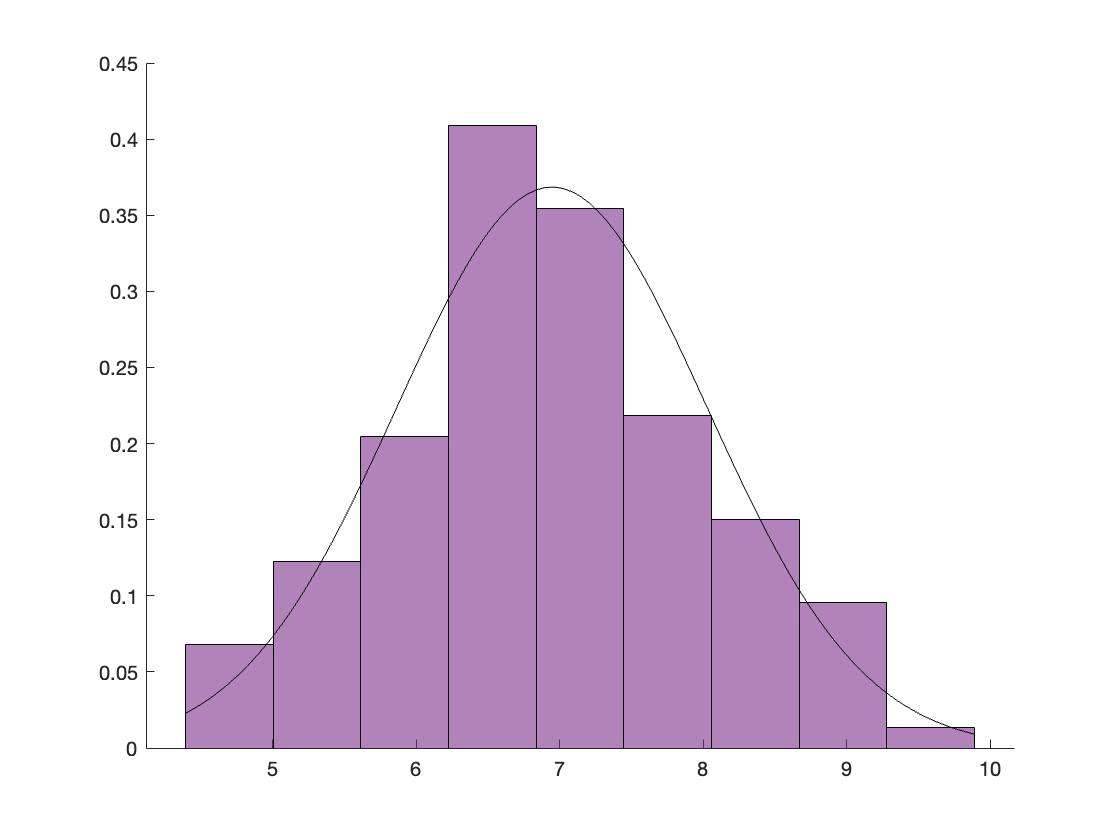
\includegraphics[width=0.7\textwidth]{images/1.png}}
 \caption{Гистограмма и график функции плотности распределения вероятностей нормальной случайной величины с математическим ожиданием $\hat\mu$ и дисперсией $S^2$}
\end{figure}

\begin{figure}[!h]
 \center{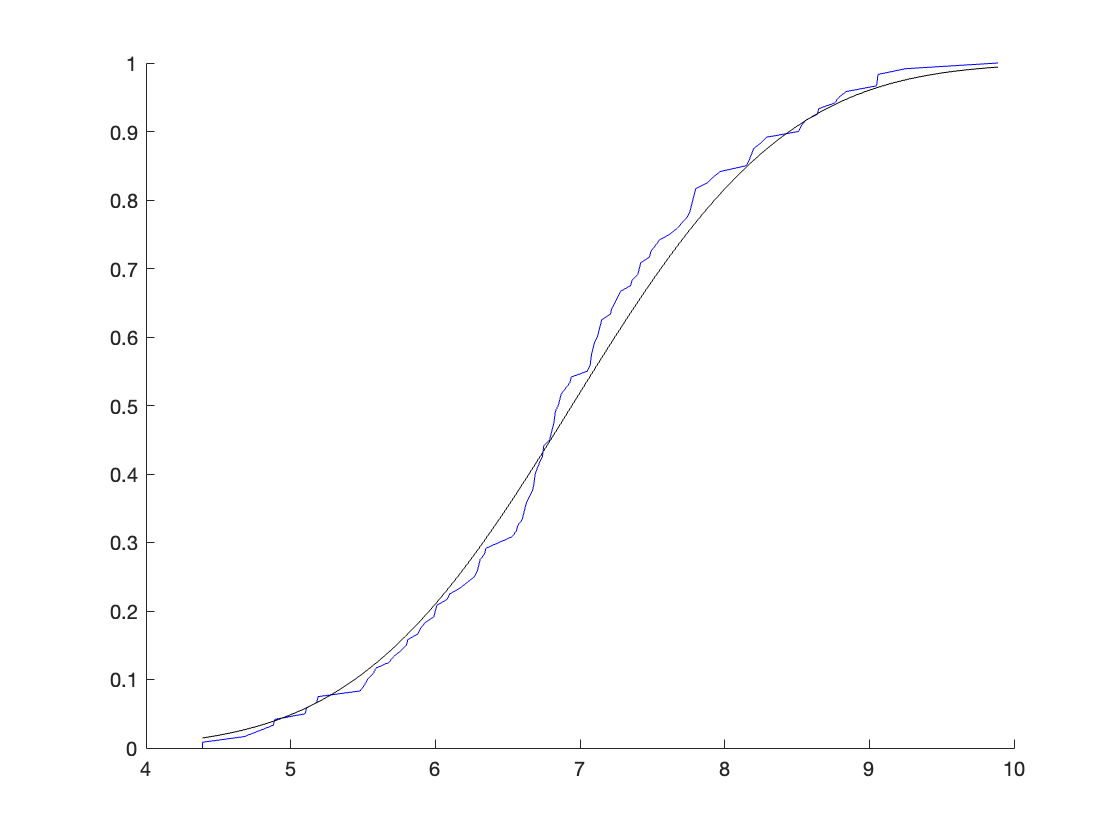
\includegraphics[width=0.7\textwidth]{images/2.png}}
 \caption{График эмпирической функции распределения и функции распределения нормальной случайной величины с математическим ожиданием $\hat\mu$ и дисперсией $S^2$}
\end{figure}



\newpage